% Created 2020-10-06 Tue 15:16
% Intended LaTeX compiler: pdflatex
\documentclass[11pt]{article}
\usepackage[utf8]{inputenc}
\usepackage[T1]{fontenc}
\usepackage{graphicx}
\usepackage{grffile}
\usepackage{longtable}
\usepackage{wrapfig}
\usepackage{rotating}
\usepackage[normalem]{ulem}
\usepackage{amsmath}
\usepackage{textcomp}
\usepackage{amssymb}
\usepackage{capt-of}
\usepackage{hyperref}
\author{adam}
\date{\today}
\title{}
\hypersetup{
 pdfauthor={adam},
 pdftitle={},
 pdfkeywords={},
 pdfsubject={},
 pdfcreator={Emacs 26.3 (Org mode 9.3.8)}, 
 pdflang={English}}
\begin{document}

\tableofcontents

\section{Computer Networks and the Internet}
\label{sec:orgb00ef5d}

\subsection{Internet overview}
\label{sec:org6f110f6}

\subsubsection{Devices}
\label{sec:org894048a}
\begin{itemize}
\item host = end system, runs apps
\end{itemize}

\subsubsection{Communication Links}
\label{sec:org681384c}
\begin{itemize}
\item fiber, copper, radio, satellite
\end{itemize}

\subsubsection{Packet switches}
\label{sec:org9ecc247}
\begin{itemize}
\item routers and switches
\end{itemize}

\subsection{Service view of the internet}
\label{sec:org141ef85}
\subsubsection{Provider of services to apps}
\label{sec:orgf6c0981}
\begin{itemize}
\item Web, VoIP, email, games, eCommerce, social net
\end{itemize}

\subsubsection{Programming interface to apps}
\label{sec:org9b25c5f}
\begin{itemize}
\item hooks
\item service options (postal)
\end{itemize}


\subsection{Protocols}
\label{sec:orga24590c}
\subsubsection{Definition}
\label{sec:org881b71d}
A protocol defines the format and the order of messages exchanged
between two or more communicating entitites, as well as the actions
taken on the transmission and/or receipt of a message or other event.

\subsubsection{Required}
\label{sec:org1c952a2}
\begin{itemize}
\item format
\item order of messages
\end{itemize}

\subsection{Network edge}
\label{sec:org7a90438}
\subsubsection{Access networks}
\label{sec:orgcef3860}
\begin{itemize}
\item Wired, wireless comms links
\end{itemize}
How does one connect an edge to a router?

\begin{itemize}
\item Frequency division multiplexing
\item Cable network is shared
\item HFC: hybrid fiber coax
\item fiber homes -> ISP router
\item DSL
\item Ethernet

\item WLAN: IEEE\textsubscript{802.11}
\end{itemize}

\subsubsection{Physical media}
\label{sec:orgec92ee9}
\begin{itemize}
\item Guided (wires)
\item Unguided (radio)
\item Physical link (transmitter, \{\$x\}, receiver)
\item Bit (propagates between)
\end{itemize}


\subsection{Network core}
\label{sec:org9292399}
\subsubsection{Interconnected routers}
\label{sec:org7dc99e4}
\begin{itemize}
\item mesh of interconnected routing packets transmitted at full link
capacity
\end{itemize}

\subsubsection{Delay, loss and throughput in Packet switched networks}
\label{sec:org6ce6f21}

\begin{itemize}
\item store and forward
\end{itemize}


\begin{verbatim}

 Source     Router    Destination
|       |____________|       |
|_______|            |_______|

   R_bps               R_bps
\end{verbatim}

L bits per packet

\begin{itemize}
\item End to end delay (assumes zero propagation delay) = 2L / R
\end{itemize}

\subsubsection{Queing, delay, loss}
\label{sec:orgaab187d}

\begin{center}
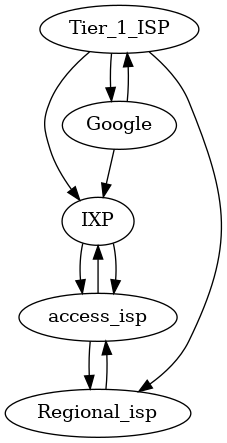
\includegraphics[width=.9\linewidth]{my-diagram.png}
\end{center}

\subsubsection{Sources of delay}
\label{sec:org9627647}
\begin{itemize}
\item transmission
\item nodal processing
\item queuing
\end{itemize}

\begin{center}
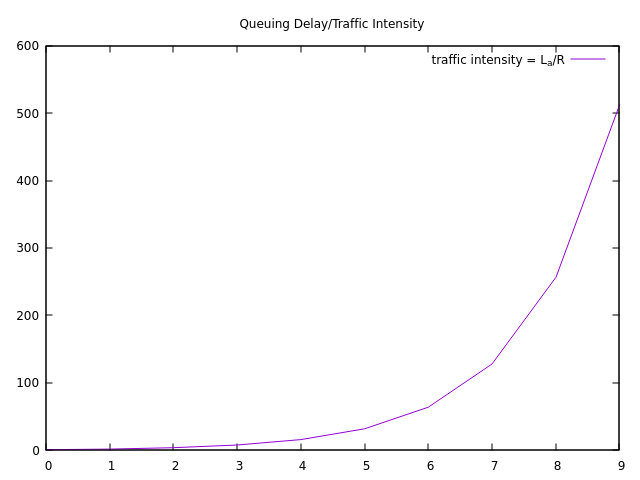
\includegraphics[width=.9\linewidth]{../img/qDelay.png}
\end{center}

\begin{center}
\begin{tabular}{rr}
traffic intensity = L\textsubscript{a}/R & Avg. queuing delay\\
1 & 0\\
2 & 1\\
4 & 2\\
8 & 3\\
16 & 4\\
32 & 5\\
64 & 6\\
128 & 7\\
256 & 8\\
512 & 9\\
\end{tabular}
\end{center}


L\textsubscript{a}/R \textasciitilde{} 0 : avg. q delay small

L\textsubscript{a}/R <= 1 : avg. q delay large

L\textsubscript{a}/R > 1 : more work arriving than can be serviced average delay
infinite

\subsubsection{Packet loss}
\label{sec:orge590d65}
Buffer has finit capacity 

packet \(\rightarrow\) full queue = dropout


\subsection{Protocol Layers}
\label{sec:org00f50c2}


\begin{center}
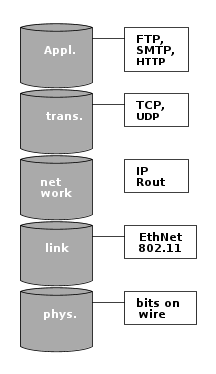
\includegraphics[width=.9\linewidth]{networklayers.png}
\end{center}

\subsubsection{iso/osi Reference Model}
\label{sec:org4fcbe7a}

Encapsulation 


\begin{verbatim}

+-------------------+ A |   | A +-------------------+
|               M   |---+   |---+                M  |
|-------------------| T |   | T |-------------------|
|           H_t M   |---+   |---+            H_t M  |
|-------------------| N |   | N |-------------------|
|       H_n H_t M   |---+   |---+        H_n H_t M  |
|-------------------| L |   | L |-------------------|
|    H_l H_n H_t M  |---+   |---+     H_l H_n H_t M |
|-------------------| P |   | P |-------------------|

\end{verbatim}

Source \(\rightarrow\)     Switch \(\rightarrow\)      Router \(\rightarrow\)     Destination 


\subsection{Network Security}
\label{sec:org2a92769}

Internet was originally designed to be used be mutuall trusting users
attached to a transparent network.

\subsubsection{Malware}
\label{sec:org9fdc944}
\begin{itemize}
\item \textbf{Virus}: self-replicating infection by receiving/executing object
(email attachment)
\item \textbf{Worm}: self-replicating infection by passively receiving object
that gets itself executed
\item \textbf{Spyware}: record keystrokes, web sites visited, upload info to
\end{itemize}

Infected host can be enrolled in botnet, used for spam. DDOS attacks.

\begin{itemize}
\item \textbf{DDOS attacks}: make resources unavailable to legitimate traffic by
overwhelming with bogus traffic
\end{itemize}

\subsubsection{Packet "sniffing" \& IP Spoofing}
\label{sec:org3cf59e2}
\begin{itemize}
\item Broadcast media
\item Promiscuous network interface reads/records all packets passing by
\item Send packet with false source address
\end{itemize}




\section{Application layer}
\label{sec:orgfe2ba04}

\subsection{Web and HTTP}
\label{sec:org86e80ba}
\subsubsection{Client-Server Architecture}
\label{sec:orgf36ffde}

\begin{center}
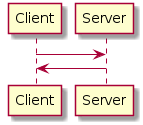
\includegraphics[width=.9\linewidth]{clientserver.png}
\end{center}

\begin{center}
\begin{tabular}{ll}
\textbf{Client} & \textbf{Server}\\
\hline
Communicates with server & Always on host\\
\hline
May be intermittantly connected & Permanent IP\\
\hline
May have dynamic IP & Data centers for scaling\\
\hline
Do not communicate directly with each other & \\
\end{tabular}
\end{center}

\subsubsection{Process Communicating}
\label{sec:orgc5c5efd}
Client process intiates comms, server process waits for contact

\subsubsection{Process}
\label{sec:orgd2bfd1d}
\begin{itemize}
\item Running within a host
\item Withing same host, two processes communicating using inter-process
communiation (defined by OS)
\item Processes in different hosts communicated by exchanging messages
\end{itemize}

\subsubsection{Sockets}
\label{sec:org3b358a4}

\begin{verbatim}

    V                  ^
+---v-----+        +---^-----+  
|_V_V_V_V_|        |_V_V_V_V_|

\end{verbatim}

\textbf{Addressing Processes}
\begin{itemize}
\item to receive messages, process must have ID
\item IP = 32 bit
\item identified = IP + Port
\item HTTP server: 80
\item Mail server: 25
\end{itemize}

\textbf{Application Layer Protocol}

Defines:
\begin{itemize}
\item dypes of messages exchanged (eg: request, response)
\item msg syntax (fields and delineation)
\item msg semantics
\end{itemize}

\subsubsection{Protocols}
\label{sec:orgc1d9073}

Open protocols:
\begin{itemize}
\item defined in RFC
\item allows for interoperatbility
\item eg: http, smtp
\end{itemize}

Proprietary protocols:
\begin{itemize}
\item eg. sype
\end{itemize}

Transport service for an app
\begin{itemize}
\item 100\% reliable?
\item can tolerate loss
\item low latency
\item multimedia, minimum throughput
\item "elastic apps" whatever throughput
\item encryption data integration
\end{itemize}

Different apps need different architecture to accommodate all user
requirements

\textbf{TCP (Transmission Control Protocol)}
\begin{itemize}
\item Reliable transport send \(\rightarrow\) receive
\item Flow control (doesn't overwhelm receiver)
\item Congestion control (throttle sender when network overloaded)
\item Does not provide: timing, minimum throughput guarantee
\item Connection oriented: setup required between client \& server process
\end{itemize}

\textbf{UDP (User Datagram Protocol)}
\begin{itemize}
\item unreliable data transfer between sending and receiving
\item does not provide: reliability, flow control, congestion control,
timing, throughput guarantee, security, or connection setup
\end{itemize}


\begin{center}
\begin{tabular}{lll}
\textbf{App} & \textbf{App layer protocol} & \textbf{underlying transport protocol}\\
\hline
email & SMTP [RFC 2821] & TCP\\
remote terminal access & Telnet [RFC 854] & TCP\\
web & HTTP [RFC 2616] & TCP\\
file transfer & FTP [RFC 959] & TCP\\
streaming & http [rtp 1889] & TCP or UDP\\
VoIP & SIP, RTP, proprietary & TCP or UDP\\
\end{tabular}
\end{center}

\subsubsection{HTTP}
\label{sec:org448b455}
HTTP is a stateless protocol, server maintains no info about previous
client requests
\textbf{uses TCP}
\begin{itemize}
\item client initiates
\item server accepts
\item http messages (application-layer protocol messages) exchanged
between browser (http client) and web server (http server)
\item TCP connection closed
\end{itemize}

\textbf{non-persistent}
\begin{itemize}
\item At most one object sent over TCP connection
\item connection then closed
\item downloading multiple objects required multiple connections
\end{itemize}

\textbf{persistent}
\begin{itemize}
\item multiple objects can be sent over single TCP connection between
client, server
\end{itemize}

\begin{center}
\includegraphics[width=.9\linewidth]{http.png}
\end{center}

\begin{center}
\includegraphics[width=.9\linewidth]{../img/http.png}
\end{center}

\subsubsection{User-server state: Cookies}
\label{sec:org1958af9}
Four components:
\begin{enumerate}
\item Cookie header line of http response message
\item cookie header line in next http request message
\item cookie file kept on user's host, managed by browser
\item backend database at website
\end{enumerate}

\textbf{uses}
\begin{itemize}
\item authentication
\item shop cart
\item recommend
\item user session state (webmail)
\end{itemize}

\textbf{cookies and privacy}
\begin{itemize}
\item permit site to learn about users
\end{itemize}

\subsubsection{Web caches (proxy server)}
\label{sec:org64d7f2b}
\begin{itemize}
\item acts as both client and server
\item typcially installed by ISP (uni, company, residential)
\item reduce response time
\item reduce traffic on access link
\end{itemize}

\subsubsection{conditional GET}
\label{sec:org2d09208}

\begin{itemize}
\item \textbf{goal}: don't send object if cache has up to date cached version
\item \textbf{cache}: specify date of cached copy in http request
\item \textbf{server}: response contains no object if cached copy up to date
\end{itemize}

\subsection{FTP}
\label{sec:org9b1a4d8}
File Transfer Protocol 

\begin{itemize}
\item to/from remote host
\item client/server model
\begin{itemize}
\item initiated by client
\item server: remote host
\end{itemize}
\item Ftp: RFC 959
\item Ftp server: port 21
\end{itemize}

\subsection{Electronic mail: SMTP, POP3, IMAP}
\label{sec:org2aee03e}
\begin{itemize}
\item User agent
\item mail server
\item SMTP
\end{itemize}

\textbf{Uses TCP on port 25}
Three phases:
\begin{itemize}
\item handshaking
\item Transfer
\item closure
\end{itemize}

\subsubsection{POP3}
\label{sec:org6de3a1d}
\begin{itemize}
\item download \& delete
\item cannot re-read file after client change
\item stateless across sessions
\item download-and-keep copies and different clients
\end{itemize}

\subsubsection{IMAP}
\label{sec:orgf058d82}
\begin{itemize}
\item keeps messages in one place:server
\item allows user to organize messages in folders
\item keeps user state accross sessions:
\begin{itemize}
\item names of folders and mappings between message IDs and folder name
\end{itemize}
\end{itemize}

\subsection{DNS}
\label{sec:org48fec2e}
Domain Name System

\begin{itemize}
\item Names map IP to readable format
\item Distributed database implemented in hierarchy of many name servers
\item application-layer protocol: hosts, name servers communicate to
resolve names (address/name translation)
\begin{itemize}
\item Note: core interenet function implemented as application-layer
protocol complexity at network's edge
\end{itemize}

\item \textbf{Root DNS Servers} over 400 worldwide (2016 numbers)
\item \textbf{Top-level domain (TLD) servers} for each of \{com, org, ned, edu,
gov, ie, at, jp, etc) there is a server or server cluster
\item \textbf{Authoratative DNS servers} publicly accessible records that map the
names of the host companies to IP addreses
\end{itemize}


\subsubsection{DNS Services}
\label{sec:org42cbe28}
\begin{itemize}
\item Hostname to IP address translation
\item host aliasing
\begin{itemize}
\item canonical alias names
\end{itemize}
\item mail server aliasing
\item load distribution 
\begin{itemize}
\item replicated web servers: many IP addresses correspond to one name
\end{itemize}
\end{itemize}

\textbf{Why not centralize DNS?}
\begin{itemize}
\item single point of failure
\item traffic volume
\item distant centralized database
\item maintenance
\item doesn't scale
\end{itemize}

\subsubsection{DNS Records}
\label{sec:orgc19003c}

DNS: distributed db storing resource records (RR) 

RR Format: (name, value, type, ttl)

\textbf{type=A}
\begin{itemize}
\item name is hostname
\item value is IP
\end{itemize}

\textbf{type=NS}
\begin{itemize}
\item name is domain
\item value is hostname of authoratative name server for this domain
\end{itemize}

\textbf{type=CNAME}
\begin{itemize}
\item name is alias for some "canonical" real name
\item www.ibm.com
\begin{itemize}
\item servereast.backup2.ibm.com
\item value is canonical name
\end{itemize}
\end{itemize}

\textbf{type=MX}
\begin{itemize}
\item value is name of mail server associated with name
\end{itemize}


\subsubsection{Attacking DNS}
\label{sec:org5c24272}

\textbf{DDoS attacks}
\begin{itemize}
\item Bombard servers with traffic
\begin{itemize}
\item Not succseful to date
\item traffic filtered
\item local DNS servers cache IPs of TLD servers, allowing root server
bypass
\end{itemize}
\item Bombard TLD (top level domain) servers
\begin{itemize}
\item potentially more dangerous
\end{itemize}
\end{itemize}

\textbf{Redirect attacks}
\begin{itemize}
\item man in the middle attacks
\begin{itemize}
\item intercept queries
\end{itemize}
\item DNS poisoning
\begin{itemize}
\item send bogus replies to DNS server, which caches
\end{itemize}
\end{itemize}

\textbf{Exploit DNS for DDoS}
\begin{itemize}
\item send queries with spoofed source address: target IP
\item requires amplification
\end{itemize}

\subsection{Principles of network applications}
\label{sec:org189379d}
\subsubsection{Server/client}
\label{sec:org038917d}
\begin{itemize}
\item send one copy F/u\textsubscript{S}
\item send N copes NF/u\textsubscript{s}
\end{itemize}

Client must download file copy
\begin{itemize}
\item d\textsubscript{min} = min client dl rate
\item min client download time: F/d\textsubscript{min}
\end{itemize}

\textbf{Distribution time}

D\textsubscript{c}-s > mac\{NF/u\textsubscript{s} , F/d\textsubscript{min}\}

\subsubsection{P2P}
\label{sec:org9fce038}

Max upload rate:  u\textsubscript{s} + \(\Sigma\) u\textsubscript{i}

distribution time (\emph{increases linearly in N}):

D\textsubscript{p2p} > max \{ F/u\textsubscript{s}, F/d\textsubscript{min}, NF/(u\textsubscript{s} + \(\Sigma\) u\textsubscript{i}) \}





\subsection{P2P Apps}
\label{sec:org2345fe7}
Commonly used to distribute software

Distributed hash table (DHT)

DHT: a distributed P2P database


\section{Transport Layer}
\label{sec:org9668efa}

\subsection{Transport Services \& Protocols}
\label{sec:org9896fbd}
\begin{itemize}
\item Provide logical communication between app processes running on
different hosts
\item Transport protocols run in and systems
\begin{itemize}
\item Send side: breaks app messages into segments, passes to network layer
\item receiveer side: reassemble segments into messages, passes to app
layer
\end{itemize}
\item More than one transport protocol available to apps
\begin{itemize}
\item Internet: TCP \& UDP
\end{itemize}
\end{itemize}

\subsection{Multiplexing and Demultiplexing}
\label{sec:orgf3b3c8e}
\begin{itemize}
\item Multiplexing at sender: handle data from multiple sockets, add
transport  header (later used for demultiplexing)
\item Demultiplexing at receiver: use header info to deliver received
segments to correct socket
\end{itemize}

\subsubsection{Port}
\label{sec:org4fcb9be}
Simply a number used by a particular software to identify its data
coming from the internet

\subsubsection{Socket}
\label{sec:orgf550826}
IP Address + Port num. Used by another computer to send data to
software on a particular machine 
\begin{itemize}
\item IP = Machine
\item Port = Software
\end{itemize}


\break

\subsection{Demultiplexing}
\label{sec:orgff95b50}

\begin{itemize}
\item Host receives IP datagrams
\begin{itemize}
\item Each datagram has source IP address, destination IP address
\item Each datagram carries one transport-layer segment
\end{itemize}
\item Host uses IP address \& port numbers to direct segment to appropriate
socket
\end{itemize}

\begin{verbatim}

<-----------32 bits--------->
+-------------+-------------+
| src port #  | dest port # |
|_____________|_____________|
|                           |
|     other header fields   |
|___________________________|
|                           |
|       application data    |   
|       payload             |
|___________________________|

\end{verbatim}
\captionof{figure}{TCP/UDP segment format}

\subsubsection{Connectionless Dmuxing}
\label{sec:orge1a0a29}
When host receives UDP segment:
\begin{itemize}
\item checks destination port number in segment
\item directs UDP segment to socket with that port number
\end{itemize}

IP datagrams with some destination port number, but different source IP
and/or source port numbers will be directed to same socket at destination.

\subsubsection{Connection-oriented Dmux}
\label{sec:orge87c716}
TCP socket identified by 4-tuple:
\begin{itemize}
\item Source IP address
\item Source port number
\item Destination IP address
\item Dest port number
\end{itemize}

Server host may support many simultaneous TCP sockets: each socket
identified by its own 4-tuple.Web servers have different sockets for
each connecting client, non persistent http will have different socket
for each request

\subsection{Connectionless Transport UDP}
\label{sec:org2800bb8}
\begin{itemize}
\item No handshaking between UDP, sender, receiver
\item each UDP segment handled independently of others
\end{itemize}

UDP uses:
\begin{itemize}
\item streaming multimedia apps (loss tolerant, rate sensitive)
\item DNS
\item best effort service
\end{itemize}

UDP segments may be
\begin{itemize}
\item lost
\item delivered out-of-order to app
\end{itemize}


\begin{verbatim}

<-----------32 bits--------->
+-------------+-------------+
| src port #  | dest port # |
|_____________|_____________|
| length      | checksum    |
|_____________|_____________|
|                           |
|     other header fields   |
|___________________________|
|                           |
|       application data    |   
|       payload             |
|___________________________|

\end{verbatim}
\captionof{figure}{UDP segment format}

\subsubsection{Why UDP?}
\label{sec:org827250a}
\begin{itemize}
\item No connection establishment (which can add delay)
\item Simple: no connection state at sender, receiver
\item Small header size
\item No congestion control: UDP can blas away as fast as desired
\end{itemize}

\subsection{Principles of Reliable Data Transfer}
\label{sec:orgfe99c1a}

\begin{figure}[htbp]
\centering
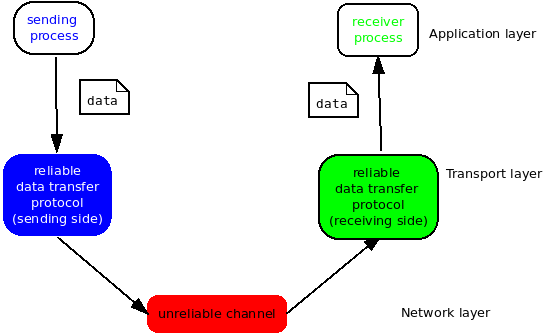
\includegraphics[width=.9\linewidth]{../img/RDT.png}
\caption{Reliable Data Transfer (RDT)}
\end{figure}

\subsubsection{RDT: Getting Started}
\label{sec:org65fb2d5}

Relies on four functions

\begin{verbatim}

rdt_send()

deliver_data()

udt_send()

rdt_rcv()

\end{verbatim}


\subsubsection{Dependency between event \& state}
\label{sec:orgd7bbe53}

\begin{figure}[htbp]
\centering
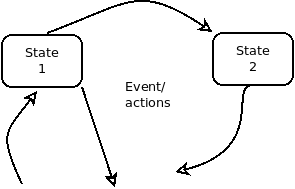
\includegraphics[width=.9\linewidth]{../img/eventStateDependency.png}
\caption{Event -><- State dependency}
\end{figure}


\subsubsection{RDT 1.0}
\label{sec:org72a0dde}
Reliable data transfer over a reliable channel. Underlying channel is
perfectly reliable
\begin{itemize}
\item no bit errors
\item no loss of packets
\end{itemize}

Seperate FSMs for sender, receiver:
\begin{itemize}
\item sender sends data into underlying channel
\item receiver reads data from underlying channel
\end{itemize}

\subsubsection{RDT 2.0}
\label{sec:org2e7451d}
Channel with bit errors: underlying channel may flip bits in packet
\begin{itemize}
\item checksum to detect bit
\end{itemize}

\textbf{Question}: How to recover from errors?

\begin{itemize}
\item Acknowledgements (ACKs): receiver explicitly tells sender that pkt
received OK
\item Negative acknowledgements (NAKs): receiver explicitly tells sender
that pkt had errors
\item Sender retransmits pkt on receipt of NAK
\end{itemize}

\textbf{FATAL FLAW}
ACK/NAK can be corrupted
\begin{itemize}
\item sender doesn't know what happened at receiver
\item can't just retransmit possible duplicate
\end{itemize}

Handling duplicates:
\begin{itemize}
\item Sender retransmits current pkt if ACK/NAK corrupted
\item Sender adds sequence number to each pkt
\item Receiver discards (doesn't deliver up) ducplicate pkt
\end{itemize}

Stop and wait:
\begin{itemize}
\item sender sends one packet, then waits for receiver to respond
\end{itemize}

\subsubsection{RDT 2.1}
\label{sec:orgb2d267a}
Sender:
\begin{itemize}
\item Seq number added to pkt
\item Two sequence numbers (0,1) will suffice
\item Must check if ACK/NAK corrupted
\item Twice as many states
\begin{itemize}
\item states must "remember" whether "expected" pkt should have sequence
number of 0 or 1
\end{itemize}
\end{itemize}

Receiver: 
\begin{itemize}
\item Must check if received packet is duplicate
\begin{itemize}
\item State indicates wheter 0 or 1 expected pkt sequence number
\end{itemize}
\end{itemize}

Note: receiver can not(!) know if its last ACK/NAK received okay at
sender 

\subsubsection{RDT 2.2: A NAK-free protocol}
\label{sec:orgdd6cc63}

+Same functionality as \textbf{RDT 2.1}, using ACKs only 
\begin{itemize}
\item Instead of NAK, receiver sends ACK for last pkt received OK
\begin{itemize}
\item receiver must explicitly include sequence number of packet being
ACKed
\end{itemize}
\item Duplicate ACK at sender results in same action as NAK: retransmit
current pkt
\end{itemize}

\subsubsection{RDT 3.0: Channels with errors and loss}
\label{sec:orgdc3d164}

\textbf{New assumption}: underlying channel can also lose packets (data,
ACKs)
\begin{itemize}
\item checksum, sequence number, ACKs, retransmission will be of help
\ldots{} but not enough
\end{itemize}

\textbf{Approach}: Sender waits reasonable amount of time for ACK
\begin{itemize}
\item retransmits if no ACK received in this time
\item if pkt (or ACK) just delayed (not lost)
\begin{itemize}
\item retransmission will be duplicate, but sequence numbers already
handles this
\item receiver must specific sequence number of pkt being ACK
\end{itemize}
\item Requires countdown timer
\end{itemize}



\begin{center}
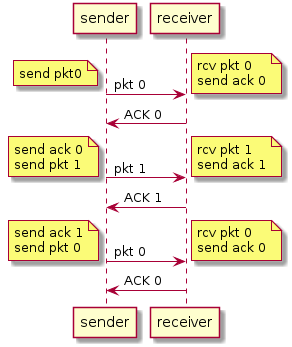
\includegraphics[width=.9\linewidth]{RDT3.0.png}
\end{center}



\subsection{Pipelined Protocols}
\label{sec:org05de6e9}

\begin{center}
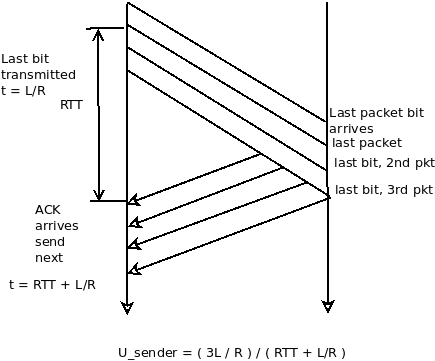
\includegraphics[width=.9\linewidth]{../img/pipelined_protocols.png}
\end{center}

\subsubsection{Got-back-N}
\label{sec:org2d28d9a}
\begin{itemize}
\item Sender can have up to N unacked packets in a pipeline
\item Receiver only sends cumulative ack
\begin{itemize}
\item doesn't ack packet if there is a gap
\end{itemize}
\item Sender has a timer for oldest unacked packet
\begin{itemize}
\item when timer expires, retransmit all unacked packtets
\end{itemize}
\end{itemize}

Packets also carry status tag, sending happens through a window

\subsubsection{Selective repeat}
\label{sec:org9fb42cb}
\begin{itemize}
\item Sender can have up to N unacked packets in a pipeline
\item Receiver sends individual ack for each packet
\item Sender maintains timer for each packet
\item When timer expires, retransmit only that unacked packet
\end{itemize}


Individual acknowledgements happen on a per packet basis

\subsection{TCP}
\label{sec:orgdb60aa9}
\subsubsection{Overview}
\label{sec:orge0ce225}
\begin{itemize}
\item RFCs: 737, 1122, 1323, 2018, 2581
\item Point to point
\begin{itemize}
\item one sender, one receiver
\end{itemize}
\end{itemize}

\subsubsection{TCP seq Number Acks}
\label{sec:org7795edc}
Sequence numbers:
\begin{itemize}
\item byte stream "number" of first byte in segment's data
\end{itemize}

Acknowledgements:
\begin{itemize}
\item Seq number of next byte expected from other side
\item cumulative ACK
\end{itemize}

\begin{center}
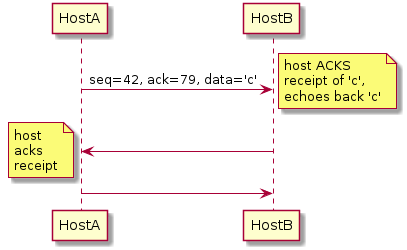
\includegraphics[width=.9\linewidth]{telnetEG.png}
\end{center}



\subsubsection{Round Trip Time, Timeout}
\label{sec:org91cd637}
\textbf{Q Set?}
\begin{itemize}
\item longer than RTT
\begin{itemize}
\item RTT varies
\end{itemize}
\item too short: premature timeout, uneccessary transmission
\item too long: show reaction to segment loss
\end{itemize}

\textbf{Estimate ?}
\begin{itemize}
\item Sample RTT: measured time from segment transmission until ACK
receipt 
\begin{itemize}
\item ignore transmissions
\end{itemize}
\item sample RTT will vary, want RTT smoother
\begin{itemize}
\item average several recent measurements
\end{itemize}
\end{itemize}


Estimated RTT = ( 1 - \(\alpha\) )*EstmiatedRTT + \(\alpha\) * SampleRTT

\subsubsection{Retransmission}
\label{sec:orgf3291e8}
\subsubsection{Flow Control}
\label{sec:orgec956ea}
\subsubsection{Connection Management}
\label{sec:org0a37350}
\subsubsection{Principles of Congestion Control}
\label{sec:orgdb5653b}
\end{document}
